% ICLR two-column figure; requires graphicx.
\begin{figure*}[t]
    \centering
    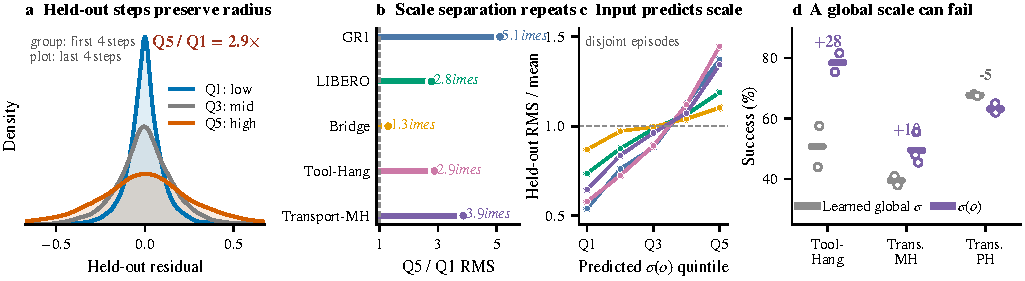
\includegraphics[width=\textwidth]{fig_hetero_necessity.pdf}
    \caption{\textbf{Robot action residuals have input-dependent scale, and one
    global scale can fail.}
    Residuals are measured against the mean action of eight nearest states from
    other episodes; binary grippers are excluded, while GR1 hand joints are
    retained. \textbf{(a)} Tool-Hang chunks grouped by first-half residual RMS
    retain separated radii over the held-out second half.
    \textbf{(b)} The held-out Q5/Q1 RMS separation repeats across five datasets
    (multi-task entries show the median task-wise ratio).
    \textbf{(c)} Under episode-level cross-fitting, query actions never enter
    their scale estimates; unseen residual RMS grows monotonically with scale
    predicted from proprioceptive state (colors follow (b)).
    \textbf{(d)} With the Student-$t$ tail and architecture fixed, $\sigma(o)$
    improves late-five success by 28 points on Tool-Hang and 10 on
    Transport-MH; Transport-PH is a negative control. Points are seeds and bars
    are means.}
    \label{fig:hetero-necessity}
\end{figure*}
